\chapter{Set Operations}

% Definition of circles
\def\firstcircle{(0,0) circle (1.5cm)}
\def\secondcircle{(0:2cm) circle (1.5cm)}
\def\universebox{ (-2,-1.75) rectangle (3.75,1.75);}

\colorlet{circle edge}{blue!50}
\colorlet{circle area}{blue!20}

\tikzset{filled/.style={fill=circle area, draw=circle edge, thick},
    outline/.style={draw=circle edge, thick}}


\newthought{There are several} ways of combining sets to produce new sets.
 
\section{Intersection}
The { \bfseries intersection} of $A$ with $B$ denoted $A\cap B$ is defined as 
$\{x | x\in A \wedge x\in B\}$.
For example $\{1,2,3,4,5\}\cap \{1,3,5,7,9\}=\{1,3,5\}$. So the intersection of 
two sets consists of the objects
which are in both sets simultaneously. Two sets are { \bfseries disjoint} if $A\cap B=\emptyset$.

\section{Venn diagrams}
Set operations can be visualized using { \bfseries Venn diagrams}. A circle (or other closed
curve) is
drawn to represent a set. The points inside the circle are used to stand for the 
elements of the set.
To represent the set operation of intersection, two such circles are drawn with an
overlap to indicate the two sets may share some elements. In the Venn diagram, figure \ref{marfig:AcapB}, 
the shaded area represents the intersection of $A$ and $B$. 

\begin{marginfigure}[-3.5cm]
% Set A intersect B
 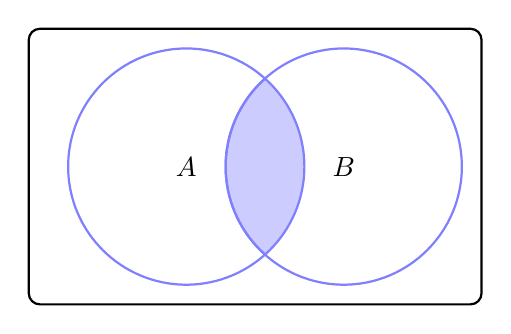
\begin{tikzpicture}
     \begin{scope}
         \clip \firstcircle;
         \fill[filled] \secondcircle;
     \end{scope}
     \draw[thick, rounded corners] \universebox
     \draw[outline] \firstcircle node {$A$};
     \draw[outline] \secondcircle node {$B$};
%     \node[anchor=south] at (current bounding box.north) {$A \cap B$};
 \end{tikzpicture}
\caption{Venn diagram for $A \cap B$}\label{marfig:AcapB}
\end{marginfigure}

\section{Union}
The { \bfseries union} of $A$ with $B$ denoted $A\cup B$ is $\{x | x\in A \vee x\in B\}$. 
In words, $A\cup B$ consists of those elements that appear in at least one of $A$ and $B$.
So for example
$\{1,2,3,4,5\}\cup \{1,3,5,7,9\}=\{1,2,3,4,5,7,9\}$. The Venn Diagram \ref{marfig:AUB}  represents
the union of $A$ and $B$.

\begin{marginfigure}[-1.5cm]
 % Set A union B
 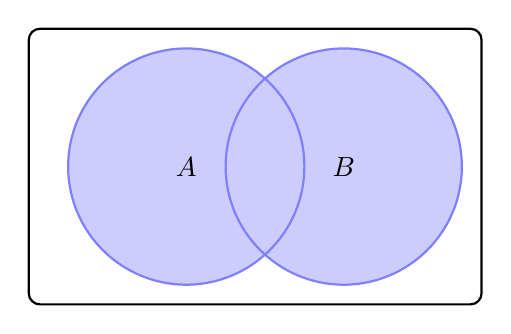
\begin{tikzpicture}
     \draw[thick, rounded corners] \universebox
     \draw[filled] \firstcircle node {$A$}
                   \secondcircle node {$B$};
%     \node[anchor=south] at (current bounding box.north) {$A \cup B$};
 \end{tikzpicture}
\caption{Venn diagram for $A \cup B$}\label{marfig:AUB}
\end{marginfigure}

\section{Symmetric difference}
The { \bfseries symmetric difference} of $A$ and $B$  is defined to be $A\oplus B = 
\{x | x\in A \oplus x\in B\}$. So $A\oplus B$ consists of those elements which appear
in exactly one of $A$ and $B$.
For example $\{1,2,3,4,5\}\oplus \{1,3,5,7,9\}=\{2,4,7,9\}$. The corresponding Venn diagram for the
symmetric difference is figure \ref{marfig:A oplus B}.

\begin{marginfigure}
%Set A or B but not (A and B) also known a A xor B
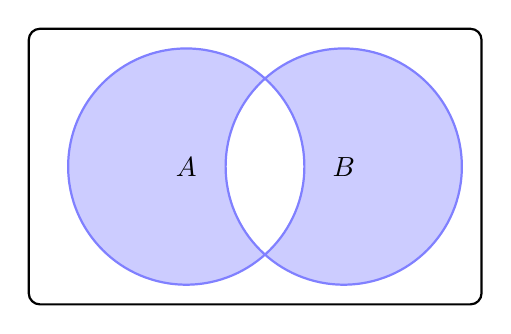
\begin{tikzpicture}
     \draw[thick, rounded corners] \universebox
    \draw[filled, even odd rule] \firstcircle node {$A$}
                                 \secondcircle node{$B$};
%    \node[anchor=south] at (current bounding box.north) {$A \oplus B$};
\end{tikzpicture}
\caption{Venn diagram for $A \oplus B$}\label{marfig:A oplus B}
\end{marginfigure}


\section{Complement}
The { \bfseries complement of} $B$ { \bfseries relative to $A$}, 
denoted $A-B$ is $\{x | x\in A \wedge x\not\in B\}$. So 
$\{1,2,3,4,5\}-\{1,3,5,7,9\}=\{2,4\}$. Figure \ref{marfig:A-B} is
the correponding Venn diagram.

\begin{marginfigure}[1.0cm]
 % Set A but not B i.e. A - B
 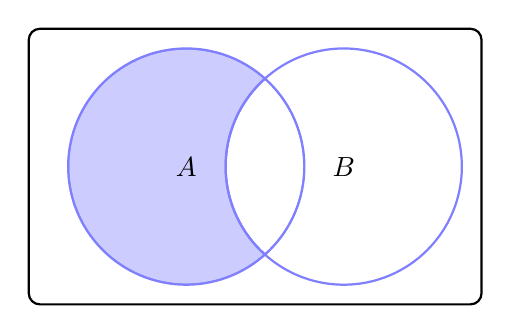
\begin{tikzpicture}
     \begin{scope}
         \clip \firstcircle;
         \draw[filled, even odd rule] \firstcircle node {$A$}
                                      \secondcircle;
     \end{scope}
     \draw[thick, rounded corners] \universebox
     \draw[outline] \firstcircle
                    \secondcircle node {$B$};
%     \node[anchor=south] at (current bounding box.north) {$A - B$};
 \end{tikzpicture}
\caption{Venn diagram for $A - B$}\label{marfig:A-B}
\end{marginfigure}



When $\U$ is a universal set, we denote $\U-A$ by $\vl{A}$ and call it the 
{ \bfseries complement} of $A$. See figure \ref{marfig:U-A} for the Venn diagram.
If $\U=\{0,1,2,3,4,5,6,7,8,9\}$, then $\vl{\{0,1,2,3,4\}}=\{5,6,7,8,9\}$. The universal 
set matters here.
If $\U=\{x\in N | x\leq 100\}$, then $\vl{\{0,1,2,3,4\}}=\{5,6,7,8,...,100\}$.

\begin{marginfigure}[1.25cm]
 % Set complement of A, i.e. U - A
 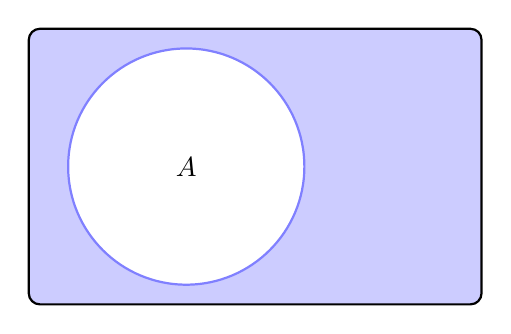
\begin{tikzpicture}
     \begin{scope}[even odd rule]
         \clip (0,0) circle (1.5cm) (-2,-1.75) rectangle (3.75,1.75);
          \fill[fill=blue!20, rounded corners] \universebox;
     \end{scope}
     \draw[thick, rounded corners] \universebox
     \draw[outline] \firstcircle node {$A$};
 \end{tikzpicture}
\caption{Venn diagram for\newline
  $\overline{A}=\mathcal{U} - A$}\label{marfig:U-A}
\end{marginfigure}

\section{Ordered lists}
The order in which elements of a set  are listed does not matter. But there are times
when order is important. For example, in a horse race, knowing the order
in which the horses cross the finish line is more interesting than simply knowing
which horses were in the race. There is a familiar way, introduced in algebra, 
of indicating order is important: ordered pairs. Ordered pairs of numbers are used to specify
points in the Euclidean plane when graphing functions. For instance, when
graphing $y=2x+1$, setting $x=3$ gives $y=7$, and so the ordered pair  $(3,7)$
will indicate one of the points on the graph. 

In this course, ordered pairs of
any sorts of objects, not just numbers, will be of interest. 
An { \bfseries ordered pair} is a collection of two objects (which might both be the
same) with one specified as first (the first coordinate) and the other as second 
(the second coordinate). The ordered pair with $a$ specified as first and $b$ as second is
written (as usual) $(a,b)$. The most important feature of ordered pairs
is that {\it $(a,b) = (c,d)$ $\iff$ $a=c$ and $b=d$}. 
In words, two ordered pairs are equal
provided they match in both coordinates. So $(1,2)\neq (2,1)$.

More generally,
an { \bfseries ordered $n$-tuple} $(a_1, a_2, ..., a_n)$ is the ordered collection 
with $a_1$ as its
first coordinate, $a_2$ as its second coordinate, and so on. Two ordered $n$-tuples are
equal provided they match in every coordinate.

\section{Cartesian product}
The last operation to be considered for combining sets is the { \bfseries Cartesian product} 
of two 
sets $A$ and $B$. It
is defined by
$\dl A\times B=\{(a,b)|a\in A\,\wedge\, b\in B\,\}.$ In other words, $A\times B$ comprises
all ordered pairs that can be formed taking the first coordinate from $A$ and the second
coordinate from $B$. 
For example if $A=\{1,2\}$, and $B=\{\alpha, \beta\}$, then 
$A\times B=\{(1,\alpha), (2,\alpha), (1, \beta), 
(2, \beta)\}$. Notice that in this case $A\times B \neq B\times A$ since, for
example, $(1,\alpha)\in A\times B$, but $(1,\alpha)\not\in B\times A$.




A special case occurs when $A=B$. In this case we denote the Cartesian product of 
$A$ with itself
by $A^2$. The familiar example $\R\times\R = \R^2$ is called the Euclidean plane or the 
Cartesian plane.

More generally given sets $A_1, ..., A_n$ the Cartesian product of these sets is written as
$A_1\times A_2\times ...\times A_n=\{(a_1, a_2,...., a_n)| a_i\in A_i, 1\leq i\leq n\}$.
Also $A^n$ denotes the Cartesian product of $A$ with itself $n$ times. 

In order to avoid the use of an ellipsis we also denote the Cartesian product of 
$A_1, ..., A_n$
as $\dl{\prod_{k=1}^n A_k}$. The variable $k$ is called the { \bfseries index} of the product.
Most often the index is a whole number. Unless we are told otherwise we start with $k=1$
and increment $k$ by $1$ successively until we reach $n$. So if we are given $A_1, A_2, A_3, 
A_4$, and $A_5$, $\dl{\prod_{k=1}^5 A_k=A_1\times A_2\times A_3\times A_4\times A_5}$.


\section{Laws of set theory}
There is a close connection between many set operations and the logical connectives
of Chapter \ref{ch:logic prop}.  The intersection operation is related to conjunction, union is related to disjunction, 
and complementation is related to negation. It is not surprising then  that the various laws of
logic, such as the associative, commutative, and distributive laws carry over to analogous
laws for the set operations. Table  \ref{tbl:laws set th}
exhibits some of these properties of these set operations. 

\begin{table}
\begin{tabular}{ll}
 \toprule
 \textbf{Identity}  & \textbf{Name}  \\ 
 \midrule
 \addlinespace
 $\vl{(\vl{A})}= A$ &Double Negation  \\ 
 \addlinespace
 $A\cap \U = A$ & \multirow{2}{*}{Identity laws}  \\ 
 $A\cup \emptyset = A$ &   \\ 
 \addlinespace 
 $A\cup \U = \U$ & \multirow{2}{*}{Domination laws} \\ 
 $A\cap \emptyset = \emptyset$ &  \\ 
 \addlinespace
 $A\cup A = A$ & \multirow{2}{*}{Idempotent laws} \\ 
 \hbox{$A\cap A= A$} &  \\ 
 \addlinespace
 $A\cup B = B\cup A$ & \multirow{2}{*}{Commutative laws} \\ 
 $A\cap B = B\cap A$ &  \\ 
 \addlinespace
 $(A\cup B)\cup C = A\cup (B\cup C)$ & \multirow{2}{*}{Associative laws} \\ 
 $(A\cap B)\cap C= A\cap (B\cap C)$ &  \\ 
 \addlinespace
 $A\cup (B\cap C)= (A\cup B)\cap (A\cup C)$ & \multirow{2}{*}{Distributive laws}  \\ 
 $A\cap (B\cup C) = (A\cap B) \cup (A\cap C)$ &  \\ 
 \addlinespace
 $\vl{(A\cap B)} = (\vl{A}\cup \vl{B})$  & \multirow{2}{*}{De Morgan's laws}  \\ 
 $\vl{(A\cup B)} = (\vl{A} \cap \vl{B})$ &  \\ 
 \addlinespace
 $A\cup \vl{A} = \U$   & Law of Excluded Middle  \\ 
 $A\cap \vl{A} = \emptyset$ & Law of Contradiction  \\ 
 \bottomrule
\end{tabular}
\caption{Laws of Set Theory}
\label{tbl:laws set th}
\end{table}

\vspace*{0.25cm}
These can be verified by using { \bfseries membership tables} which are the analogs of truth
tables used to verify the logical equivalence of propositions. For a set $A$ either an element 
under consideration
is in $A$ or it is not. These binary possibilities are kept track of using $1$ if 
$x\in A$ and $0$ if $x\not\in A$,
and then performing related bit string operations. 


\begin{exmp}
Verify the De Morgan's law given by $\vl{(A\cap B)}=\vl{A}\cup \vl{B}$.
\begin{table}
\centering
\begin{tabular}{cc|c|c|c|c|c}
$A$ & $B$ & $A\cap B$ & $\vl{(A\cap B)}$ & $\vl{A}$ & $\vl{B}$ & $\vl{A} \cup \vl{B}$ \\
\hline
1   &  1   &  1  &  0 & 0 & 0 & 0 \\
1   &  0   &  0  &  1 & 0 & 1 & 1 \\
0   &  1   &  0  &  1 & 1 & 0 & 1 \\
0   &  0   &  0  &  1 & 1 & 1 & 1 
\end{tabular}
\end{table}

The meaning of the first row of the table  is that if $x\in A$ and $x\in B$, then $x\not\in\overline{A\cap B}$,
as indicated by the $0$ in the first row, fourth column, and also not in $\overline{A}\cup\overline{B}$
as indicated by the $0$ in the first row, last column. Since the columns for  $\overline{A\cap B}$
and $\overline{A}\cup\overline{B}$ are identical, it follows that 
$\overline{(A\cap B)}=\overline{A}\cup \overline{B}$ as promised.
\end{exmp} 


\section{Proving set identities}
Just as compound propositions can be analyzed using truth tables, more complicated combinations of
sets can be handled using membership tables.  For example, using a membership table, it is easy
to verify that $\vl{A\cup(B\cap C)} = \vl{A}\cap({\vl{B}\cup\vl{C}})$. But, just as with 
propositions, it is usually more enlightening to verify such equalities by applying the few
basic laws of set theory listed above.

\begin{exmp}
Let's prove $\vl{A\cup(B\cap C)} = \vl{A}\cap({\vl{B}\cup\vl{C}})$
\begin{proof}
 The proof is just two applications of De Morgan's laws:
\[
  \vl{A\cup(B\cap C)} = \vl{A} \cap (\vl{B\cap C})  = \vl{A} \cap (\vl{B}\cup\vl{ C}).
\]
\end{proof}
\end{exmp}


\section{Bit string operations}
There is a correspondence between set operations of finite sets and bit string
operations. Let $\U=\{u_1, u_2, ..., u_n\}$ be a finite universal set with distinct 
elements listed in a specific  order\sidenote{Notice the universal set is \textbf{ordered}. We may write it as and $n$-tuple: $\U=(u_1, u_2, ..., u_n)$.}
For a set $A$ under consideration, we have $A\subseteq \U$. By the law of excluded 
middle, for each $u_j\in \U$,
either $u_j\in A$ or $u_j\not\in A$. We define a binary string of length $n$, called 
the { \bfseries characteristic vector}\label{defn:char vector}
of $A$, denoted $\chi(A)$, by setting the $j$th bit of $\chi(A)$ to be $1$ if $u_j\in A$ 
and $0$ if $u_j\not\in A$.
For example if $\U=\{1,2,3,4,5,6,7,8,9\}$, and $A=\{1,3,4,5,8\}$, then $\chi(A)=101110010$. 

An interesting side-effect is that for example $\chi(A\cap B)=\chi(A)\wedge \chi(B)$ %
\sidenote{As a function, we say that $\chi$ maps intersection to conjunction},
$\chi(A\cup B)=\chi(A)\vee \chi(B)$ and $\chi(\vl{A})=\neg \chi(A)$. Since 
every proposition can be expressed using $\wedge, \vee$ and $\neg$, 
if we represent sets by their characteristic vectors, 
we can get a machine
to perform set operations as logical operations on bit strings. This is the method programmers use
to manipulate sets in computer memory.

\clearpage



\section{Exercises}

\begin{exer}
Let $A=\{2,3,4,5,6,7,8\}$ and $B=\{1,2,4,6,7,8,9\}$. Find 
\begin{tasks}(3)
	\task $A\cap B$
	\task $A\cup B$
	\task $A-B$
	\task $B-A$
\end{tasks}
\end{exer}

\begin{exer}
Determine the sets $A$ and $B$, if $A-B=\{1,2,7,8\}$,\newline
$ B-A=\{3,4,10\}$ and $A\cap B=\{5, 6, 9\}$.
\end{exer}

\begin{exer}
Use membership tables to show that \newline
 $A\oplus B=(A\cup B)-(A\cap B)$.
\end{exer}

\begin{exer}
Verify $A \oplus B = (A\cup B) - (A \cap B)$ using Venn diagrams.
\end{exer}

\begin{exer}
Verify $A\cup(A\cap B) = A$ using the rules of set algebra.
\end{exer}

\begin{exer}
Let $A=\{1,2,3,4\}, B=\{a, b, c\}, C=\{\alpha, \beta\}, $ and $D=\{7,8,9\}$.
Write out the following Cartesian products.
\begin{tasks}(3)
	\task $A\times B$
	\task $B\times A$
	\task $C\times B\times D$
\end{tasks}
\end{exer}

\begin{exer}
What can you conclude about $A$ and $B$ if $A\times B = B\times A$.
\end{exer}

\begin{exer}
If $\U=\{0,1,2,3,4,5,6,7,8,9\}$, determine $\chi(\{1,2,4,8\})$.
\end{exer}

\begin{exer}
Let $A = \{1,2,3\}\times\{1,2,3,4\}$. List the elements in the set $B = \{(s,t)\in A\,|\, s\geq t\}$.
\end{exer}


\clearpage
\section{Problems}

\begin{prob}
Let $A=\{1,2,3,5,6,7,9\}$ and $B=\{1,3,4,6,8,9\}$. Find 
\begin{tasks}(2)
\task $A\cap B$
\task $A\cup B$
\task $A-B$
\task $B-A$\\[5pt]
\end{tasks}
\end{prob}

\begin{prob}
Use the rules of set algebra to verify $A\oplus B=(A\cup B)-(A\cap B)$.
\end{prob}


\begin{prob}
Let $A=\{1,2,3\}\times\{1,2,3,4\}$. List the elements of the set
$B= \{ (s,t)\in A\,|\, s< t\,\}$. 
\end{prob}

\begin{prob}
Let $A=\{0,1,2,3,4,5,6,7,8,9\}\times\{0,1,2,3,4,5,6,7,8,9\}$. 
  \begin{tasks}
      \task What is the cardinality of $A$? 
      \task What is the cardinality of $A\times A$?
      \task What is the cardinality of $B= \{ s\,|\, (s,s^2)\in A\,\}$?
  \end{tasks}     
\end{prob}

\begin{prob}
True or False:
   \begin{tasks}
      \task For all sets $A,B,C$, $A\times(B\cap C) = (A\times B)\cap(A\times C)$.
      \task For all sets $A,B,C$, $A\times(B\cup C) = (A\times B)\cup(A\times C)$.
      \task For all sets $A,B,C,D$, $(A\cap B)\times(C\cap D) = (A\times C)\cap(B\times D)$.
      \task For all sets $A,B,C,D$, $(A\cup B)\times(C\cup D) = (A\times C)\cup(B\times D)$.
    \end{tasks}
\end{prob}

\begin{prob}
Let $\U = \{ 1, 2, 3, 4, 5, 6, 7, 8\}$.  Find $\chi(\{1, 2, 3, 4\})$.
\end{prob}

 

